\section{Preliminary Results from Belle Open Data}

\subsection{Charged hadron multiplicity distributions}

Figure~\ref{fig:multPID} shows the multiplicity distribution of identified hadrons (pions, kaons and protons) obtained after 
applying the selection on the particle transverse momentum (0.1 $<p_{\rm T}<$ 4.0 GeV/$c$). 
The dominant contribution to the total event multiplicity is coming from pions as expected.
In Fig.~\ref{fig:multHadron}, the charged hadron multiplicity distribution $N$ is shown. The multiplicity distribution is smooth and the largest raw particle multiplicity observed in these events is about 70 before corrections for tracking efficiency, misidentification and multiple reconstruction rates, which is large given the relatively low center-of-mass energy of the collisions. Detailed studies of primary vertex-track matching and track quality as well as possible pile-up event rejection are needed for the full Belle data analysis and those effects could lower the significance of the possible correlation signals.

\begin{figure}[!htb]
\begin{center}
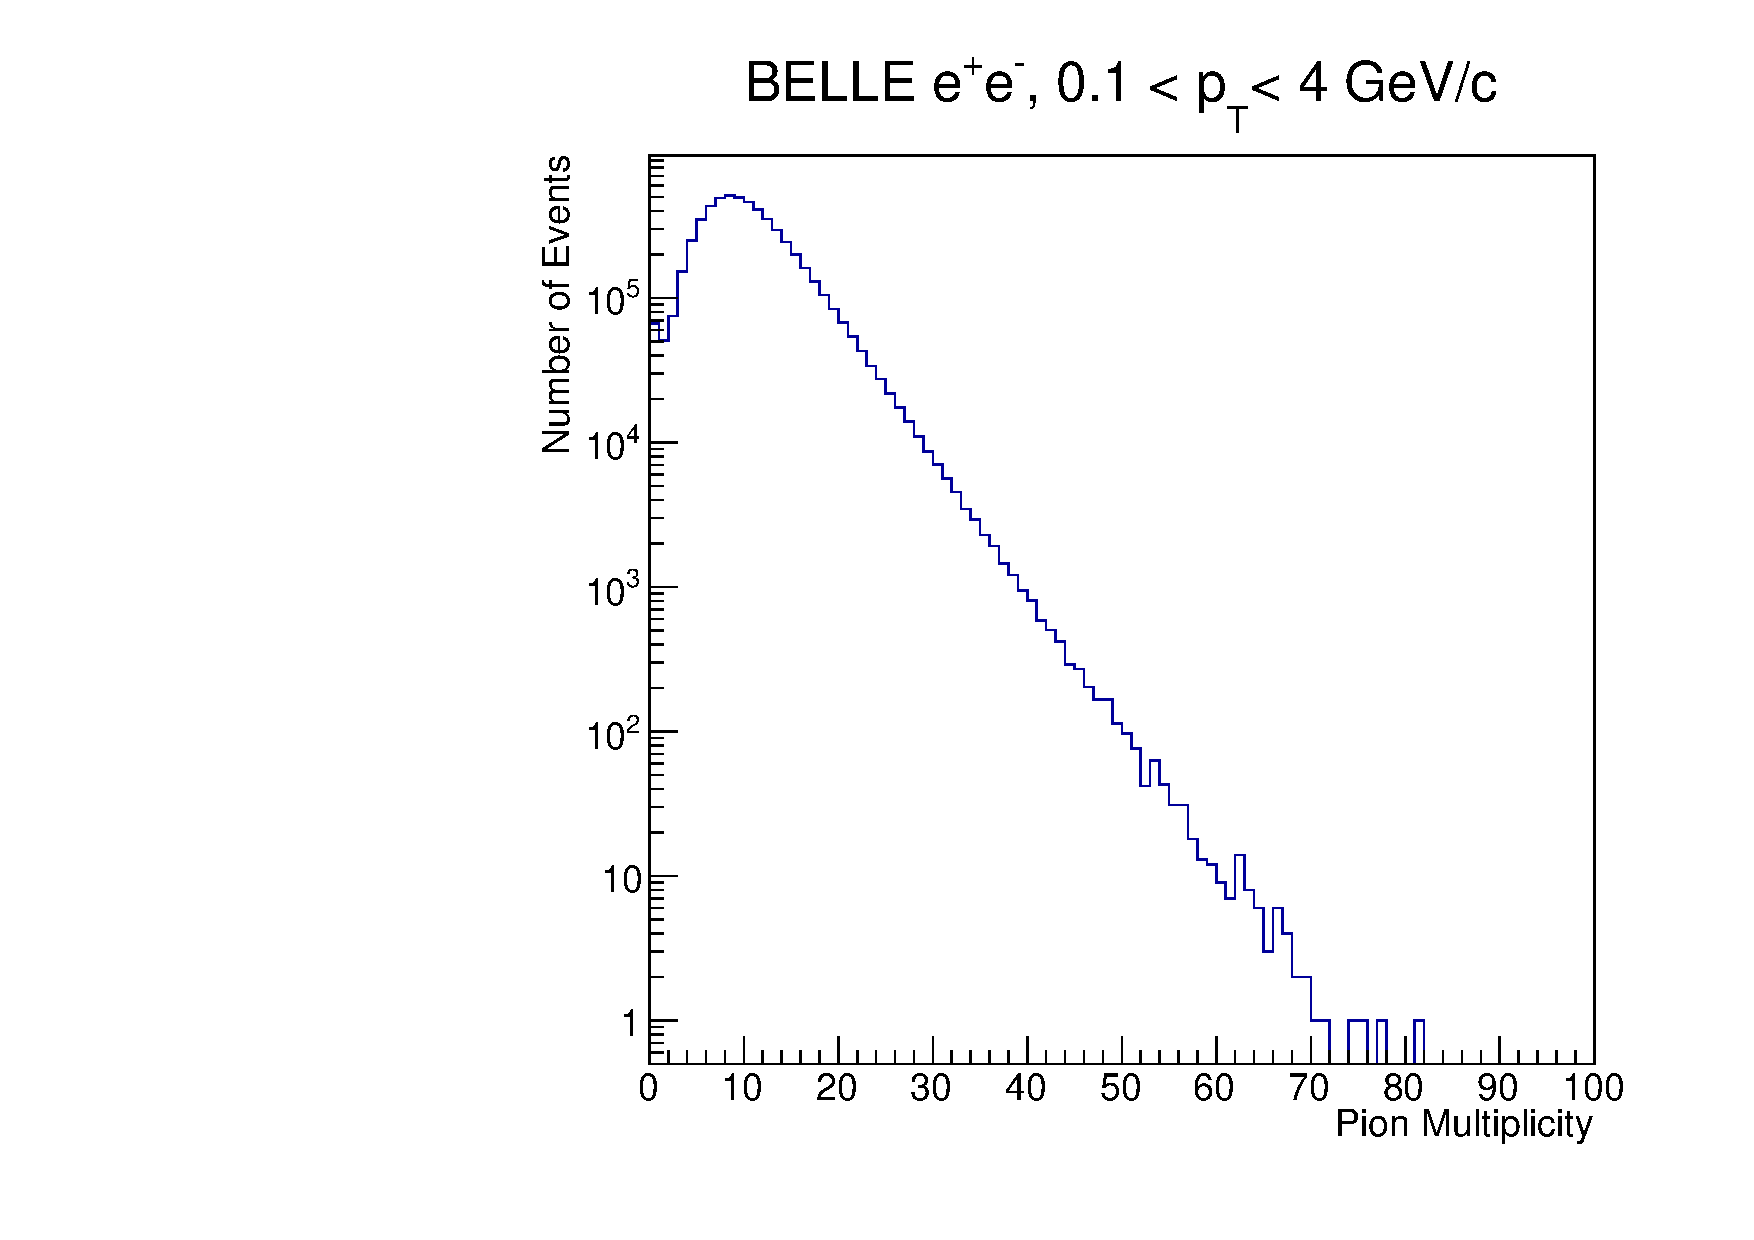
\includegraphics[width=.32\textwidth]{figures/pion_mult.pdf}
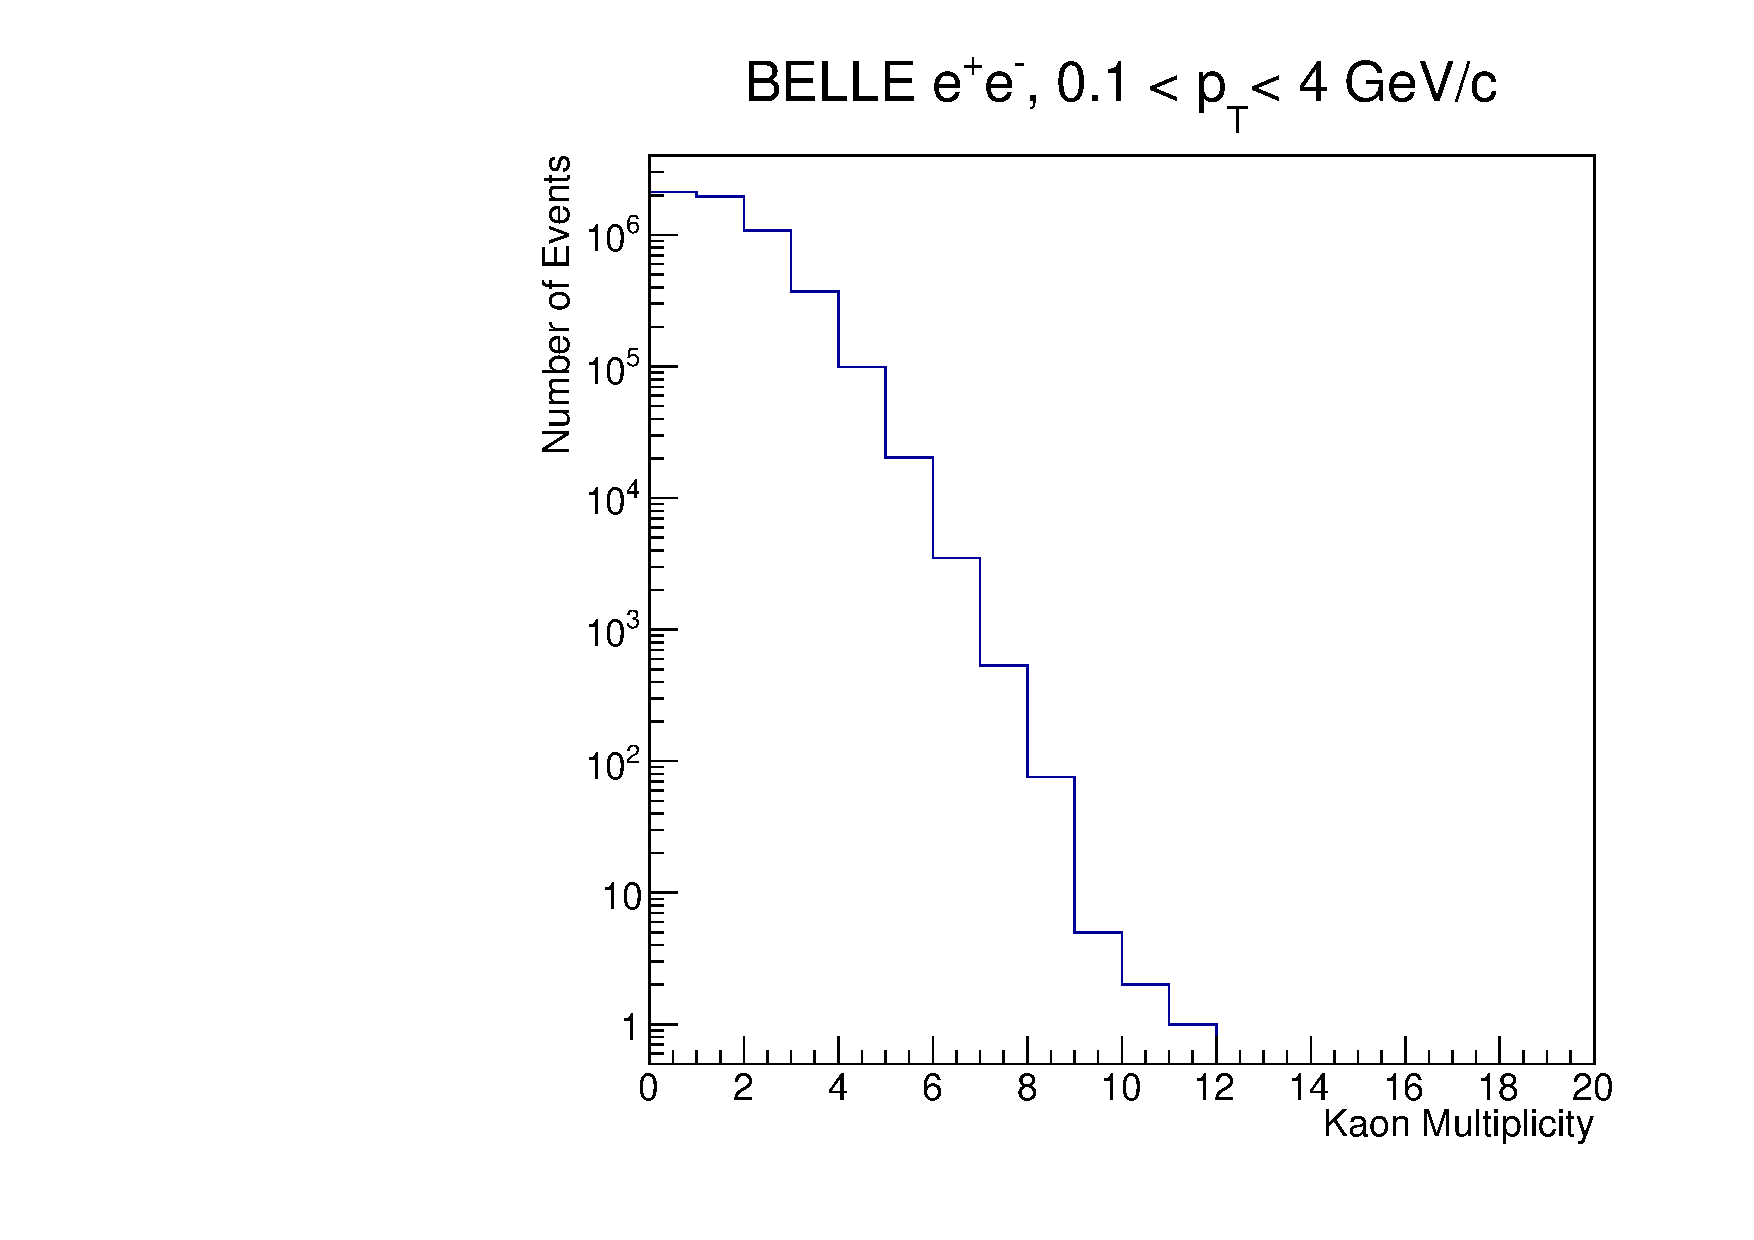
\includegraphics[width=.32\textwidth]{figures/kaon_mult.pdf}
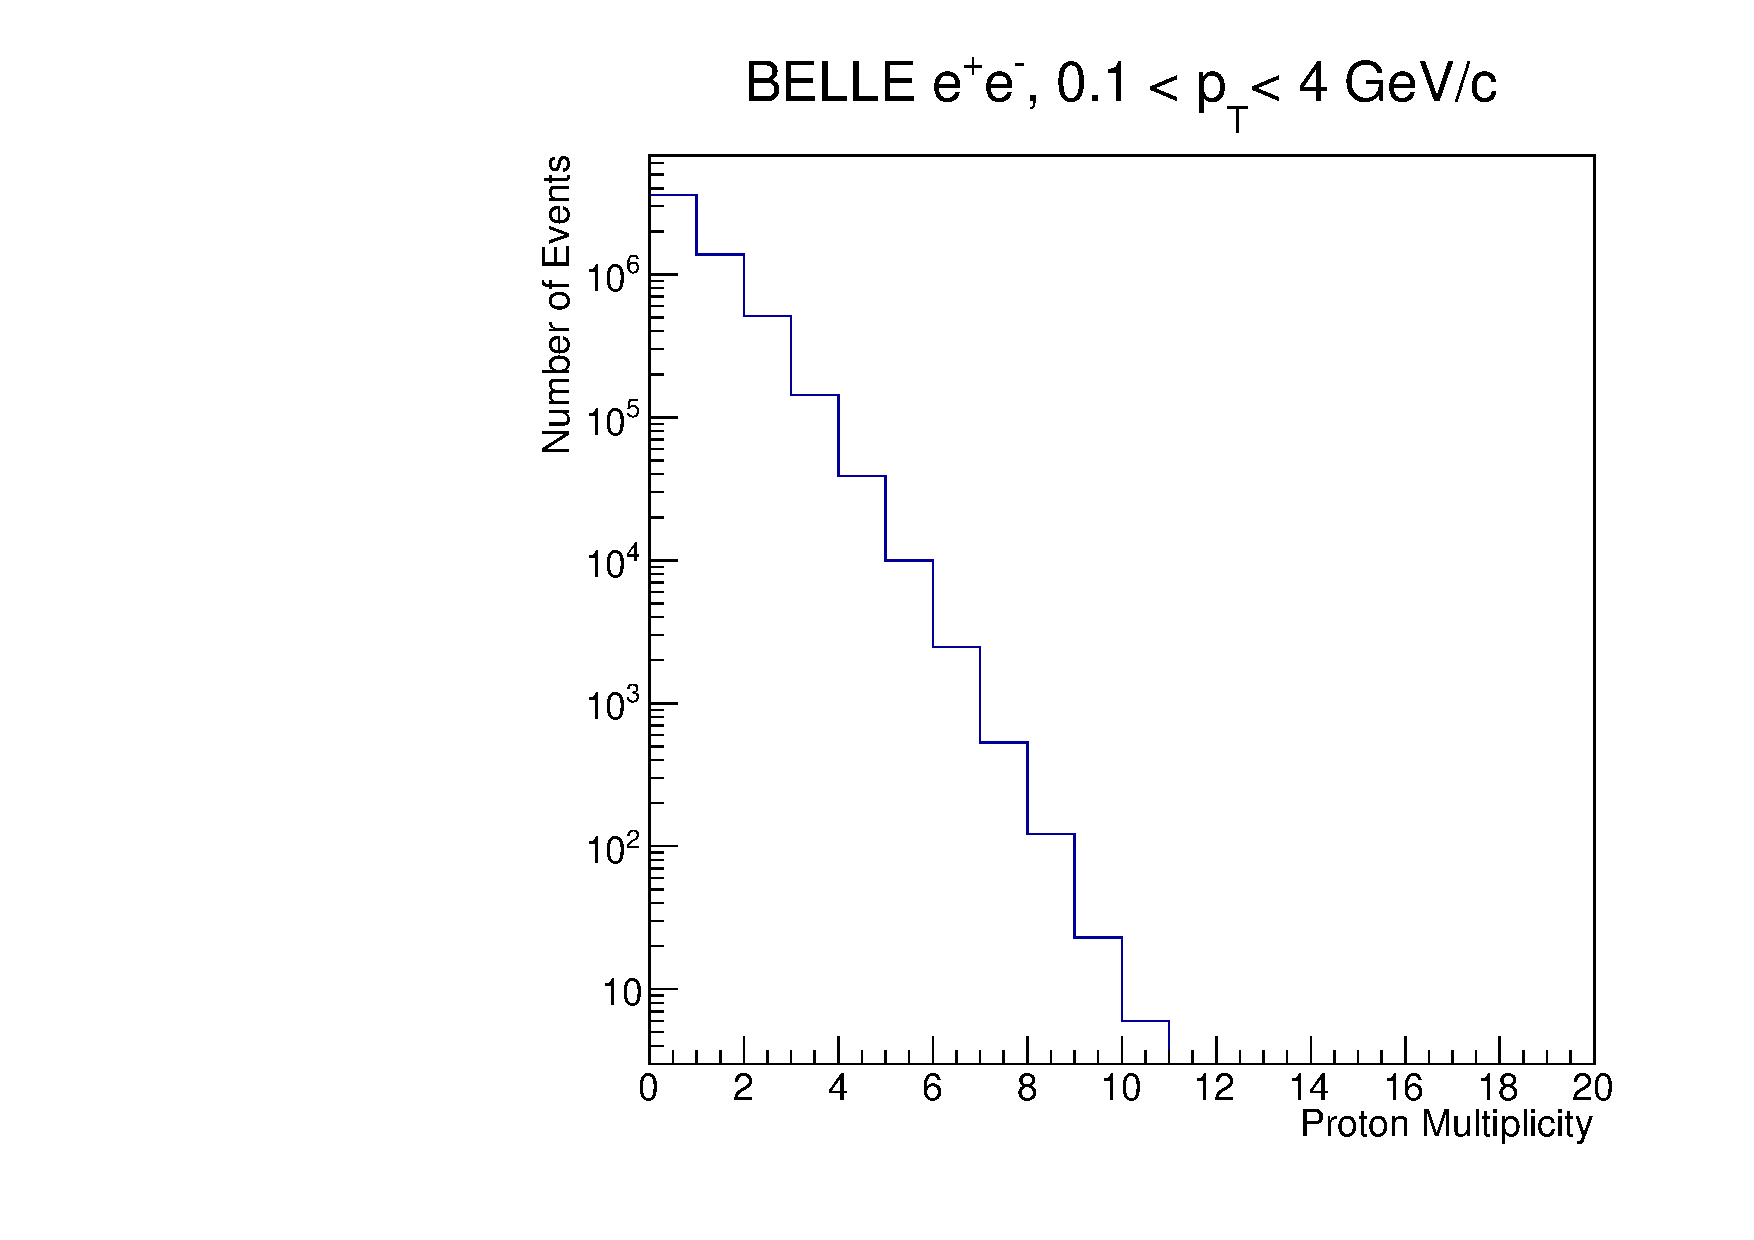
\includegraphics[width=.32\textwidth]{figures/proton_mult.pdf}
\caption{Uncorrected multiplicity distributions of pions (left), kaons (middle), protons (right) for  particles in the range  0.1 $<p_{\rm T}<$ 4.0 GeV/$c$ in $e^{+}e^{-}$ collisions. }
\label{fig:multPID} 
\end{center}
\end{figure}

\begin{figure}[!htb]
\begin{center}
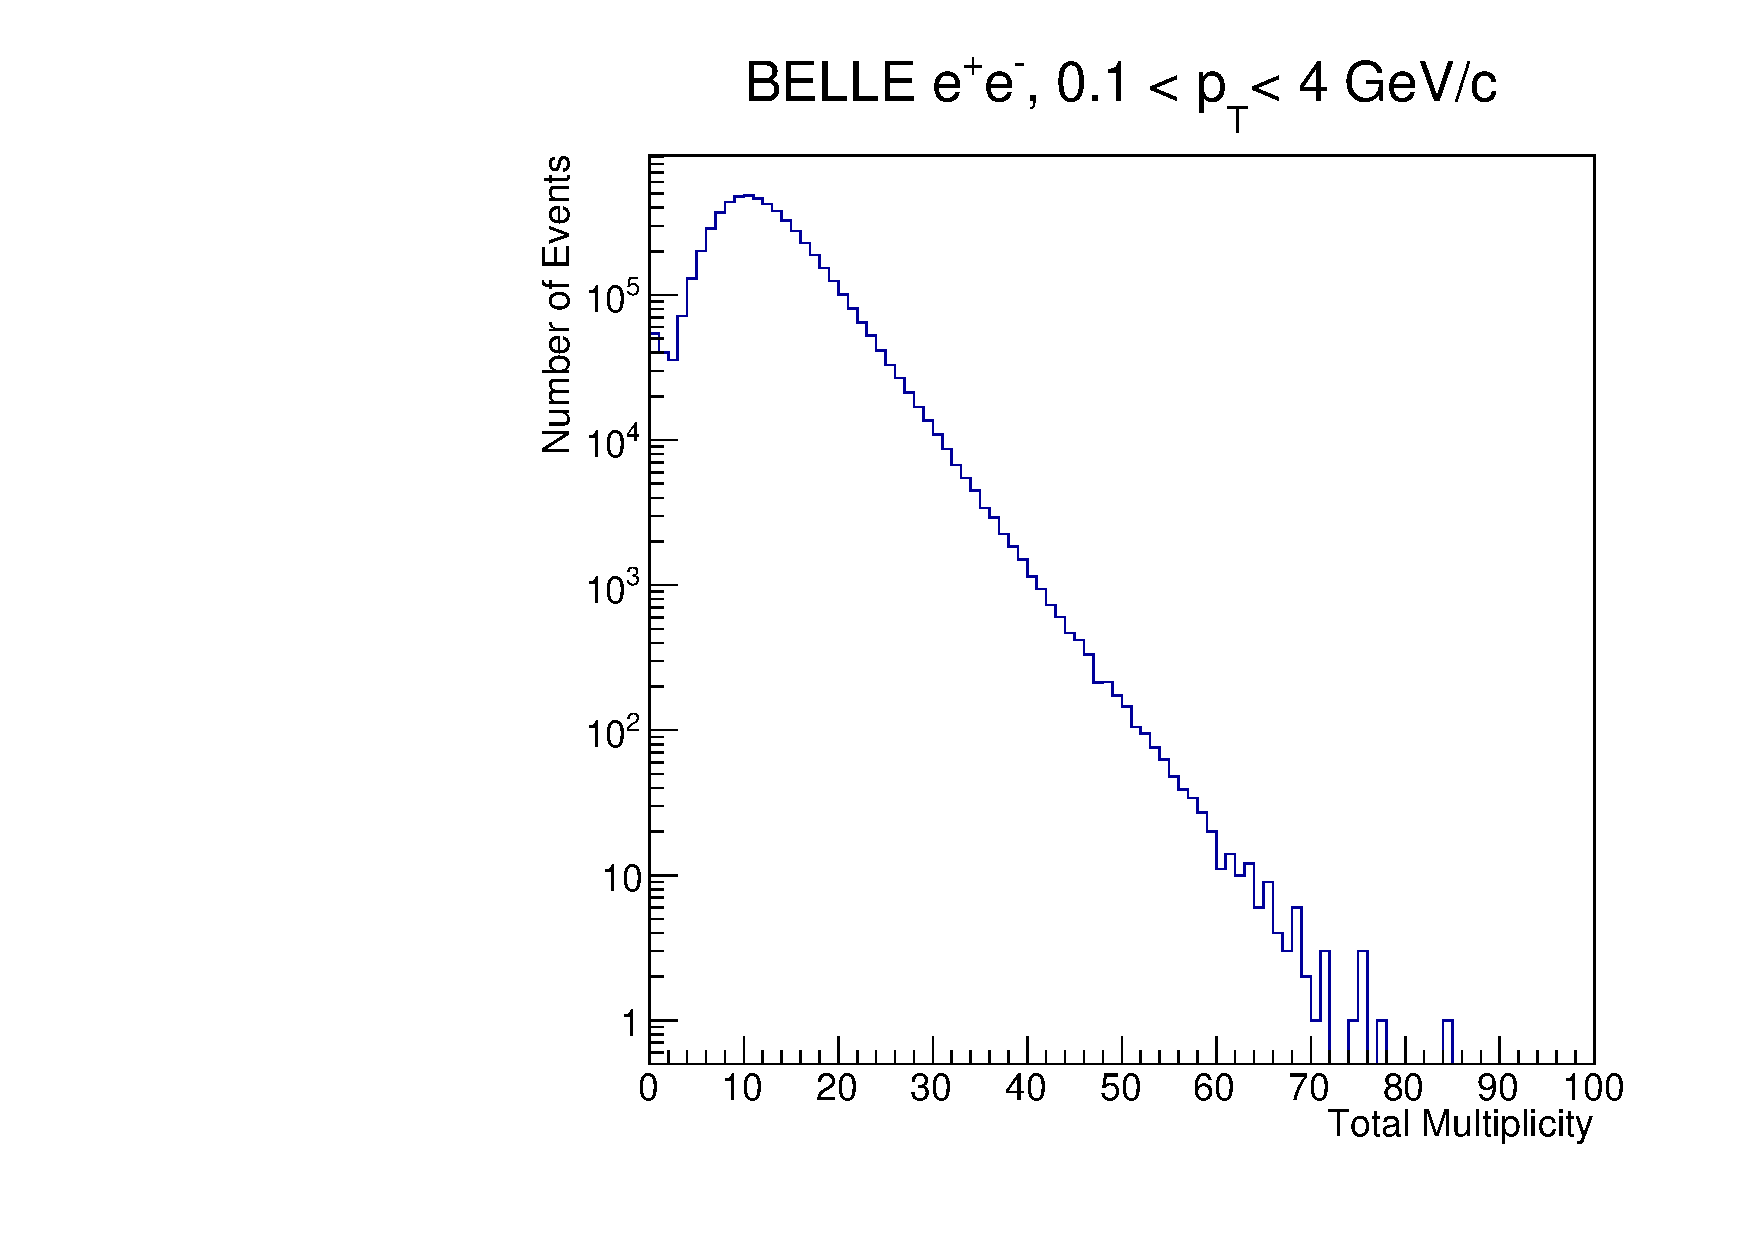
\includegraphics[width=.45\textwidth]{figures/total_mult.pdf}
\caption{Multiplicity distribution of charged hadrons (protons, kaons and pions) for  particles in the range  0.1 $<p_{\rm T}<$ 4.0 GeV/$c$ in $e^{+}e^{-}$ collisions. }
\label{fig:multHadron} 
\end{center}
\end{figure}

\subsection{Two-particle correlation functions}

In Fig.~\ref{fig:ridgeBelle}, the two-particle correlation functions from low (N$>$20) and high multiplicity (N$>50$) events are presented. In low-multiplicity events, the dominant features of the correlation function are the jet peak near $(\Delta\eta,\Delta\phi)=(0,0)$ for pairs of particles originating from the same jet and the elongated structure at $\Delta\phi\sim\pi$ for pairs of particles from back-to-back jets. %To better illustrate the full correlation structure, the jet peak has been truncated in the high multiplicity event.
The same-side jet peak and back-to-back correlation structures are also observed in high multiplicity events. 
In addition, a hint of ``ridge"-like structure is visible at $\Delta\phi \sim$0 in the right panel of Fig.~\ref{fig:ridgeBelle}. 

To separate and inspect the long-range and short-range structure, one-dimensional distributions in $\Delta\phi$ are obtained by integrating over two $|\Delta\eta|$ intervals: 0$<|\Delta \eta|<$1 and 
2$<|\Delta \eta|<$3.  At small $\Delta\eta$, a near-side peak at $\Delta\phi=$0 and the contribution from the back-to-back jet at $\Delta\phi=\pi$ is observed in the left panel of Fig~\ref{fig:ProjectionMult50}. At large $\Delta\eta$, a near-side peak at $\Delta\phi=0$ is shown in the right panel of Fig~\ref{fig:ProjectionMult50}, similar to the structures observed in high multiplicity pp, pA and AA collisions over a wide range of energies. However, the significance of this signal is limited by the available statistics in the Belle open data. This motivates a detailed study with the high statistics hadronic data taken by the Belle collaboration. 

\begin{figure}[!htb]
\begin{center}
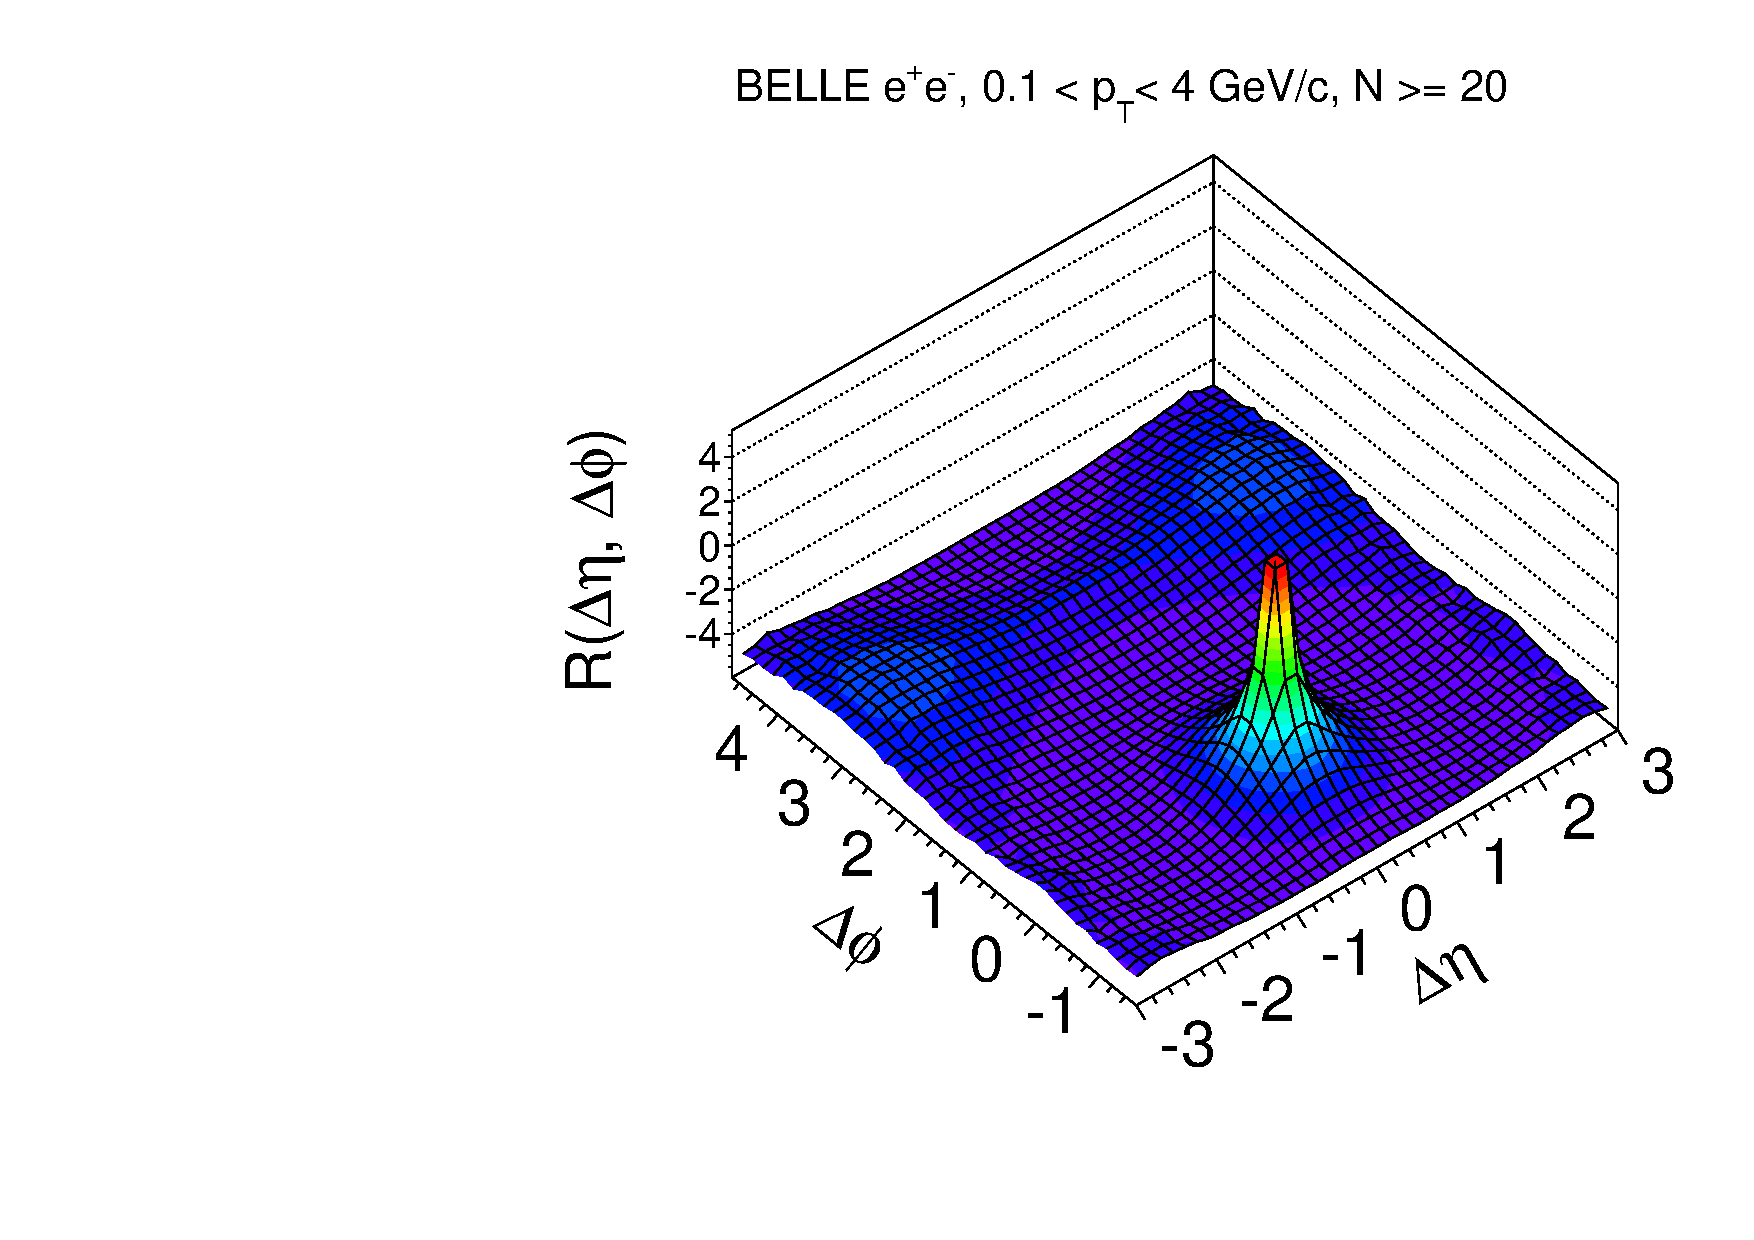
\includegraphics[width=.45\textwidth]{figures/canvasRidgeBelleMult20CutHigh0.pdf}
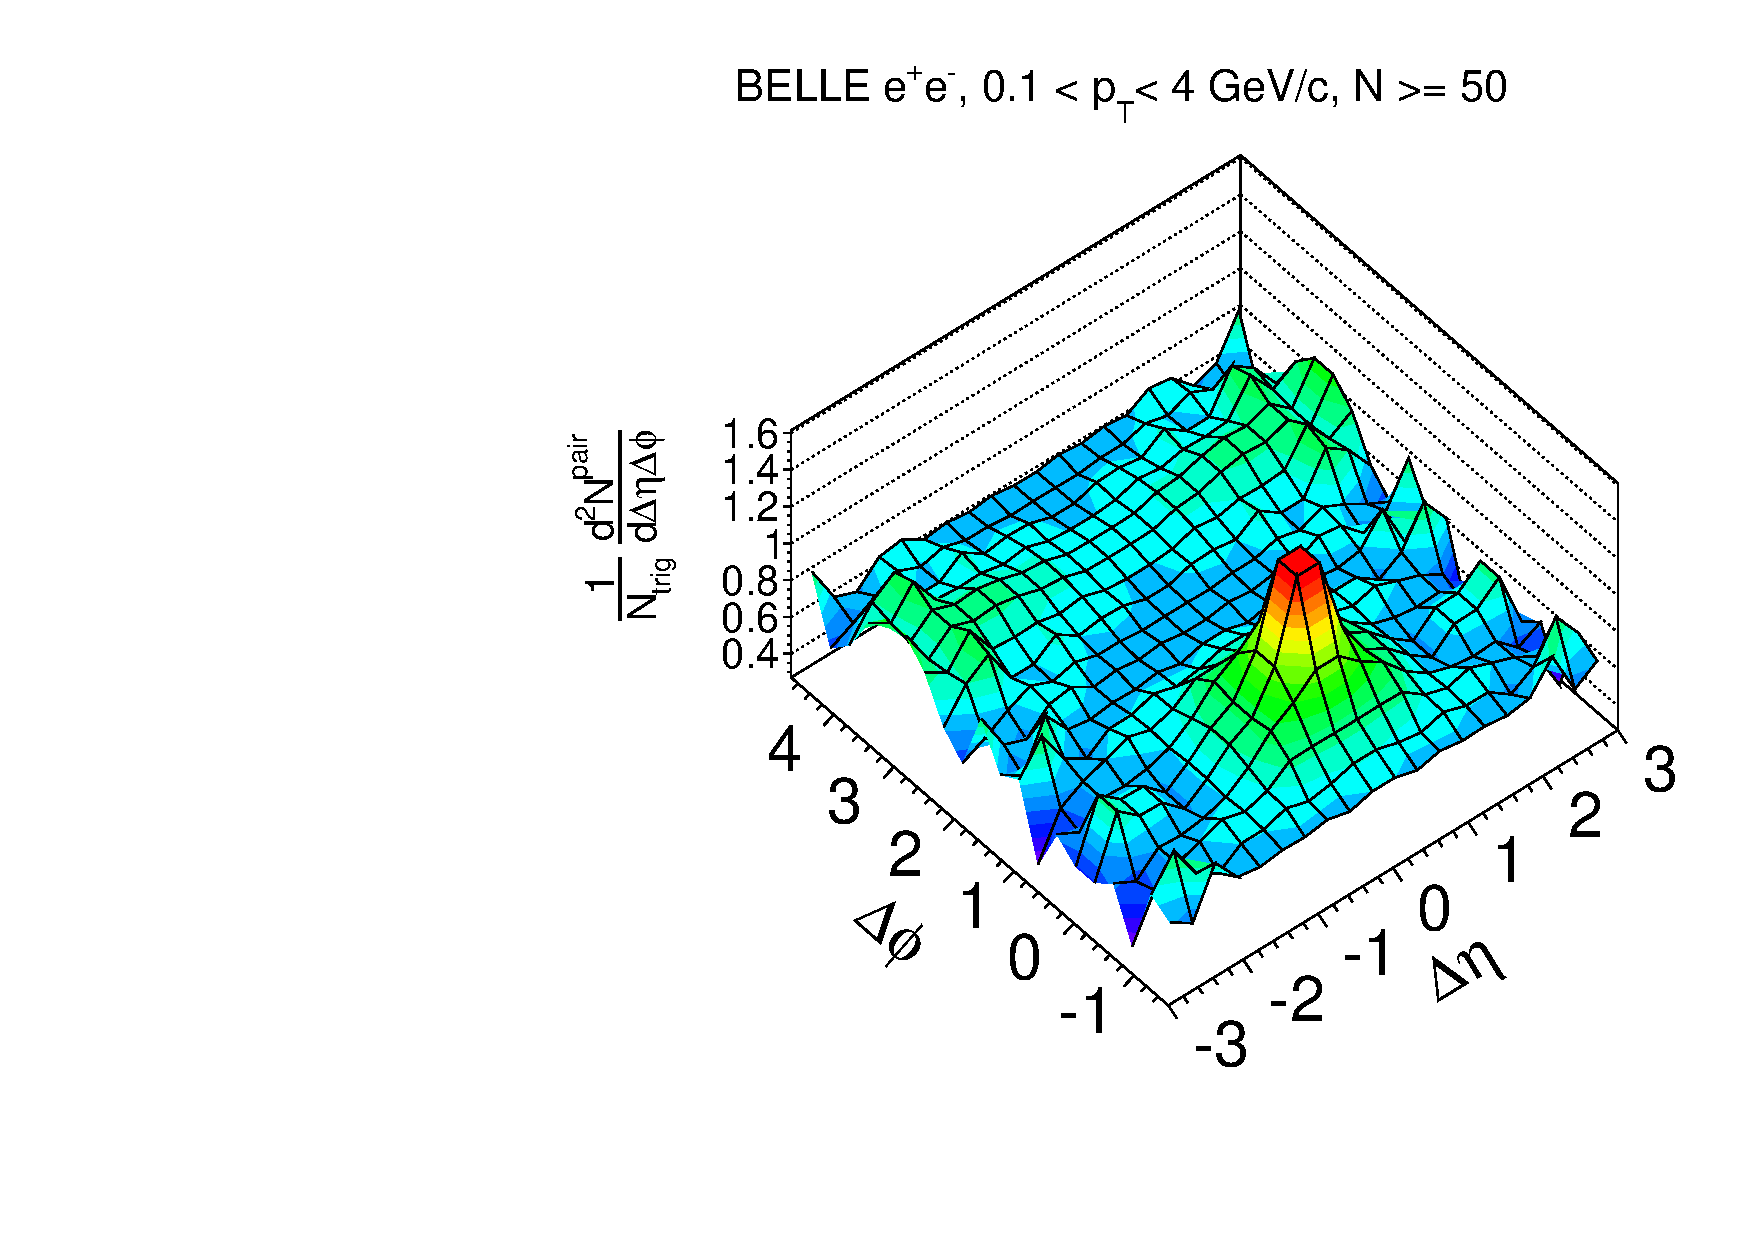
\includegraphics[width=.45\textwidth]{figures/canvasRidgeBelleMult50CutHigh0.pdf}
\caption{Two-particle correlation functions versus $\Delta\eta$ and $\Delta\phi$ in $e^{+}e^{-}$ collisions for events with particle multiplicity $>$ 20 (left) and  $>$ 50 (right).}
\label{fig:ridgeBelle} 
\end{center}
\end{figure}

\begin{figure}[!htb]
\begin{center}
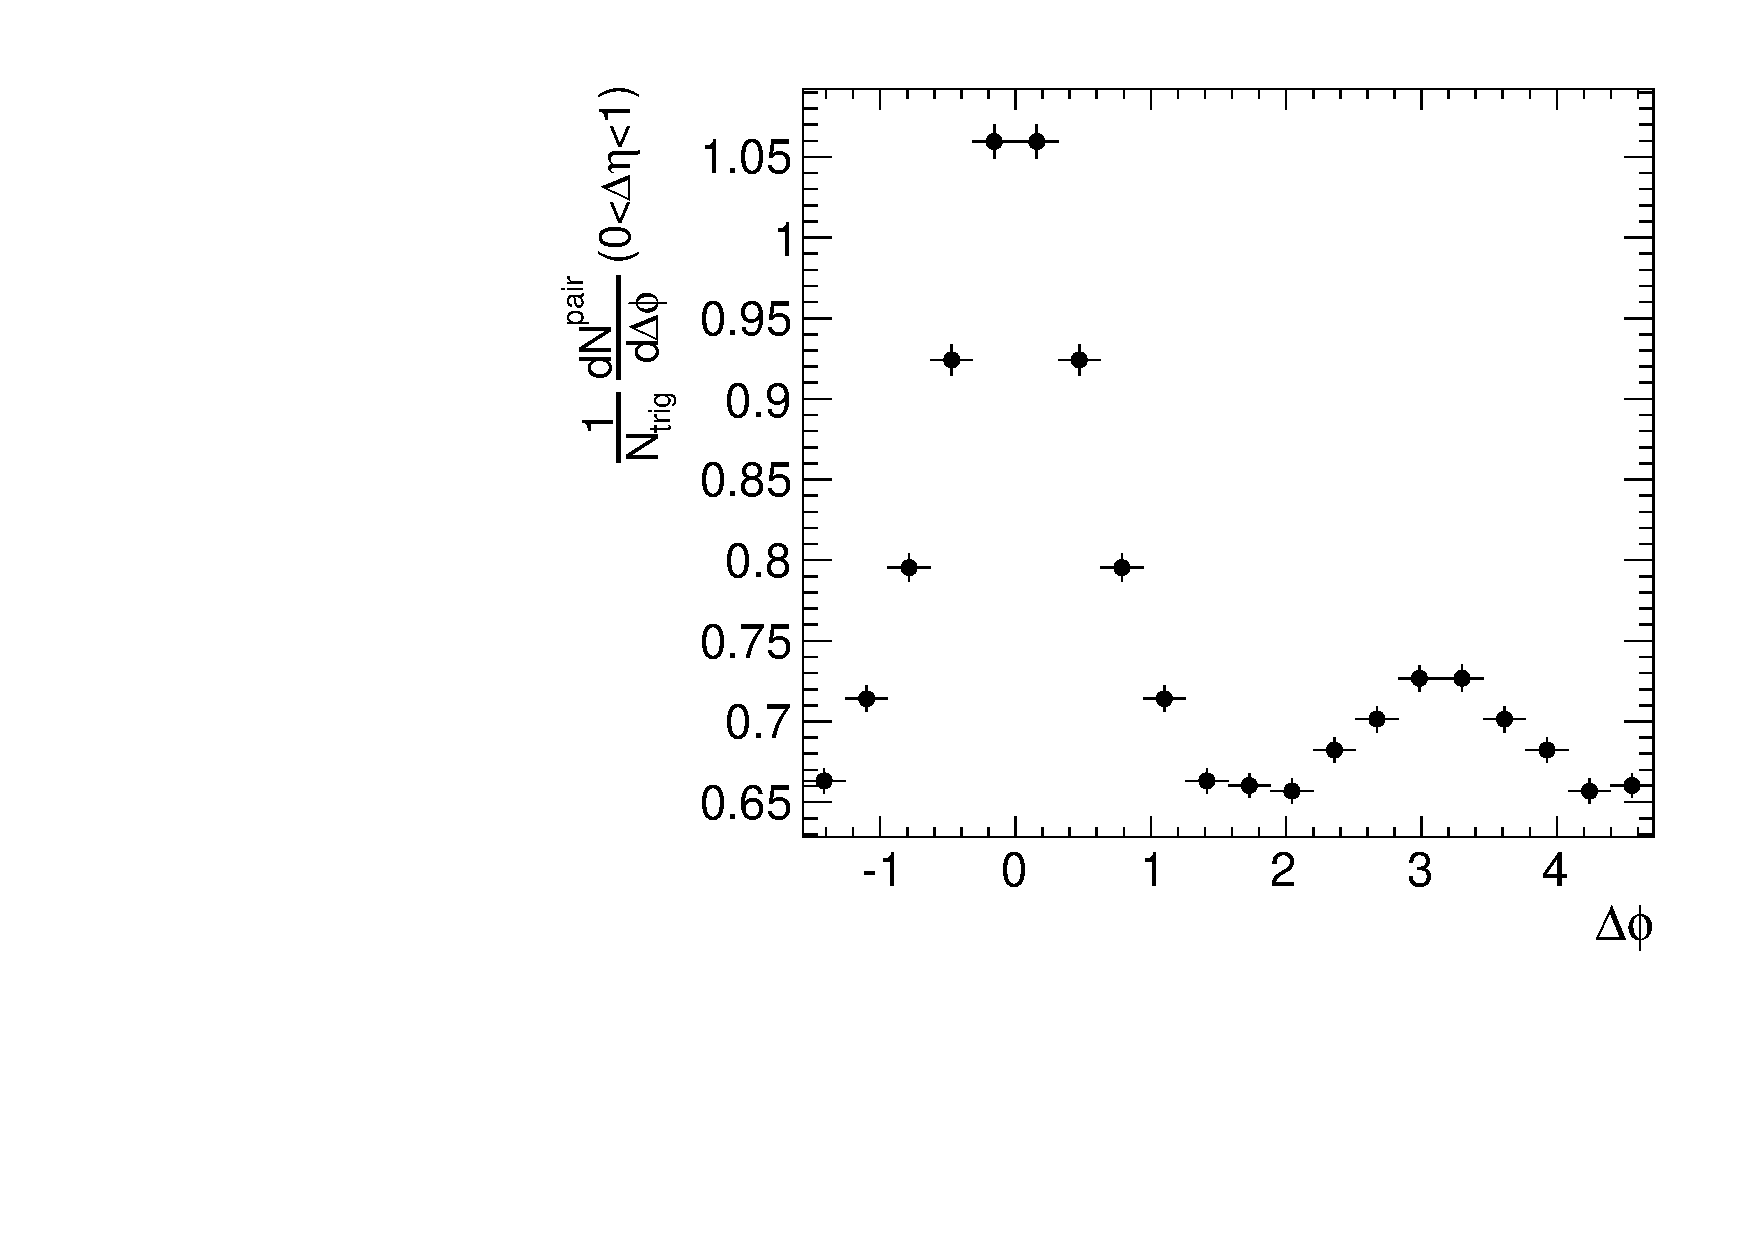
\includegraphics[width=.45\textwidth]{figures/canvasProjection_isBelle1_mult50_eta01.pdf}
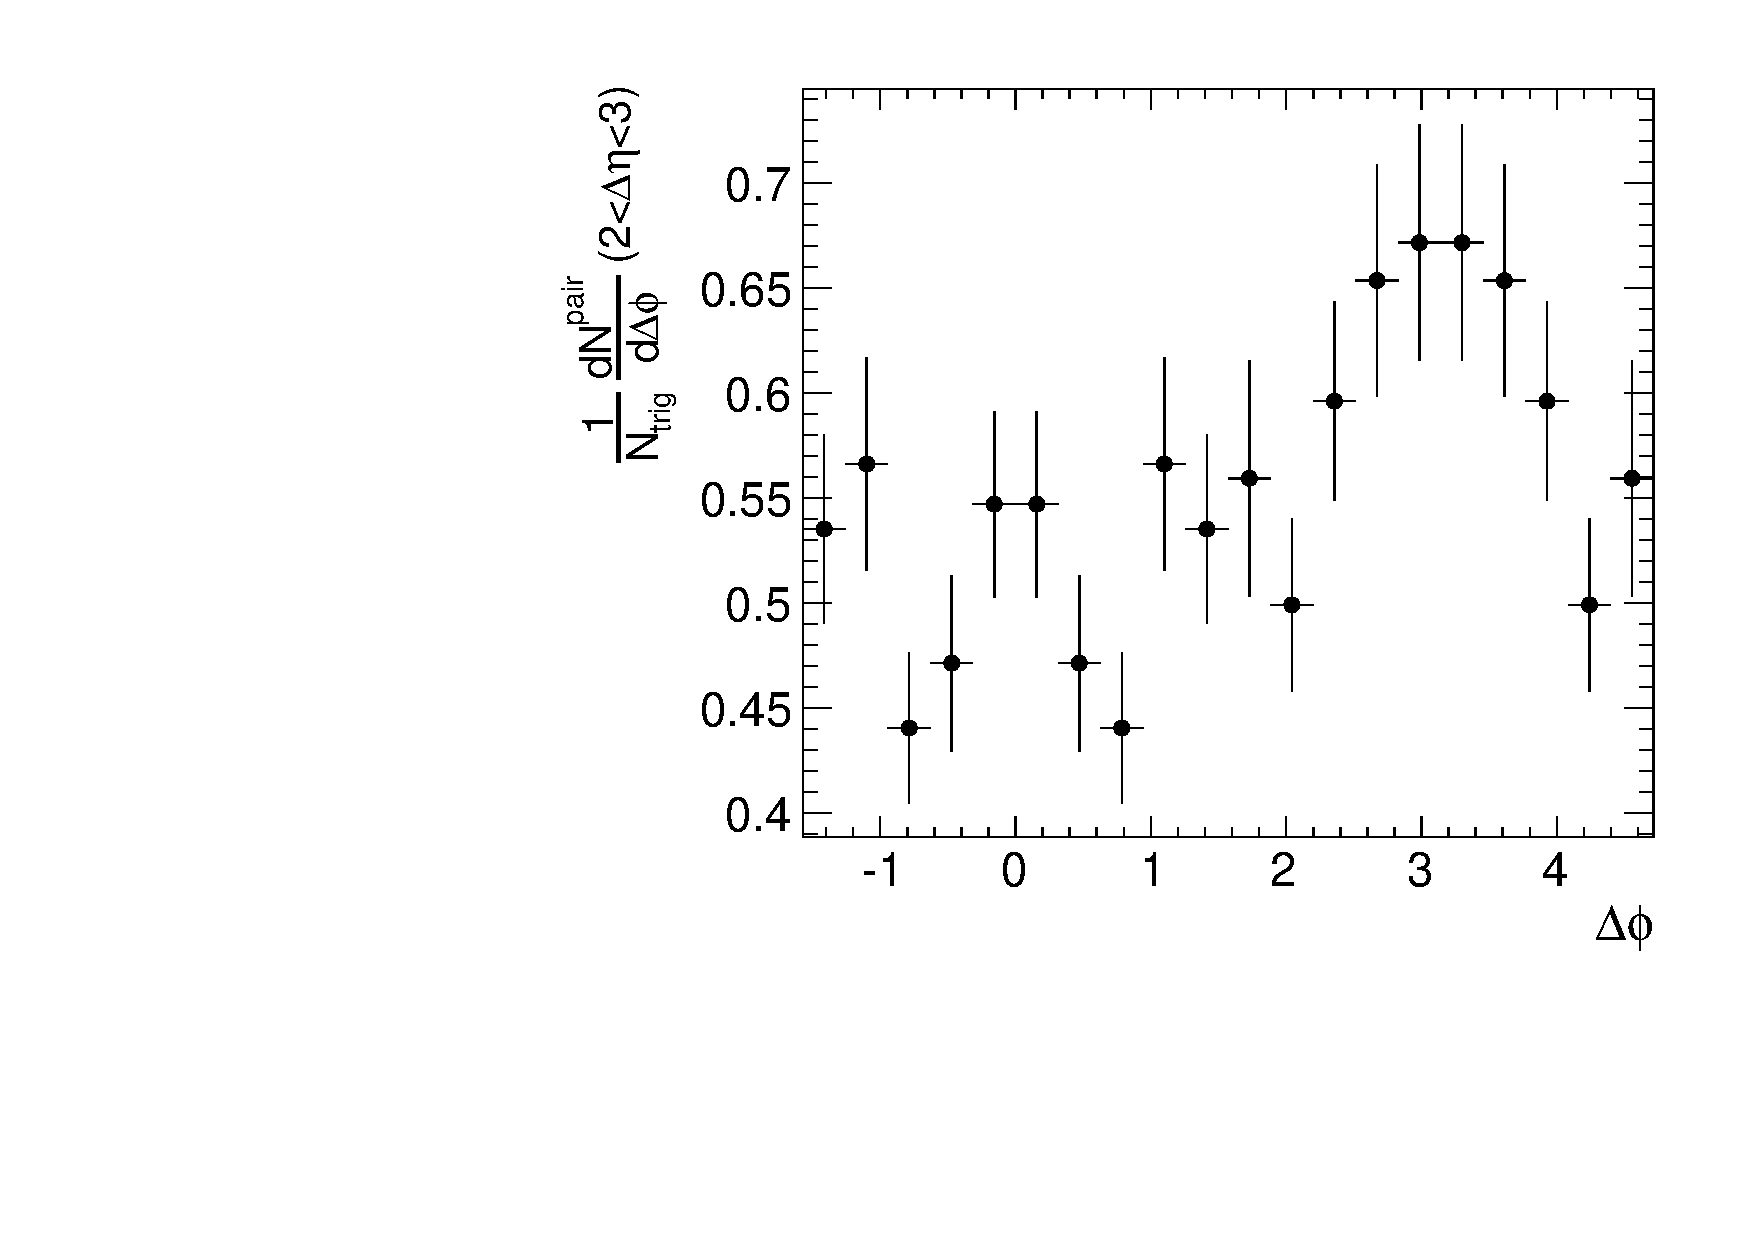
\includegraphics[width=.45\textwidth]{figures/canvasProjection_isBelle1_mult50_eta23.pdf}
\caption{Two-particle correlation functions as a function of  $\Delta\phi$ in $e^{+}e^{-}$ in the pseudorapidity ranges 0$<\Delta \eta<$1 (left) and 2$<\Delta \eta<$3 (right) for events with particle multiplicity $>$ 50.}
\label{fig:ProjectionMult50} 
\end{center}
\end{figure}

